\documentclass[11pt]{article}
\usepackage[T1]{fontenc}
\usepackage[utf8]{inputenc}
\usepackage{lmodern}
\input{glyphtounicode}
\pdfgentounicode=1
\usepackage{amsmath,amssymb,amsthm,geometry,hyperref,tikz}
\usepackage[title]{appendix}
\geometry{margin=1in}
\emergencystretch=1em
\hypersetup{colorlinks=true,linkcolor=blue,citecolor=blue,urlcolor=blue,pdftitle={Fathi's consecutive-integers bound does not extend to multitwists},pdfauthor={P. Graham},pdfsubject={Dehn multitwists and pseudo-Anosov mapping classes},pdfkeywords={mapping class group, Dehn twist, multitwist, pseudo-Anosov, Ivanov's problems, Lean}}
\newtheorem{theorem}{Theorem}
\newtheorem{lemma}[theorem]{Lemma}
\newtheorem{question}[theorem]{Question}
\theoremstyle{remark}
\newtheorem{remark}[theorem]{Remark}
\newcommand{\Mod}{\mathrm{Mod}}
\newcommand{\Z}{\mathbb{Z}}
\newcommand{\file}[1]{\texttt{\detokenize{#1}}}
\newcommand{\doi}[1]{\href{https://doi.org/#1}{doi:#1}}
\title{Fathi's consecutive-integers bound does not extend to multitwists}
\author{P. Graham\\ \small\url{https://orcid.org/0009-0007-8493-1505}}
\date{October 25, 2026}
\begin{document}
\maketitle
\begin{abstract}
On the sphere with five boundary components, a fixed positive
multitwist can have exceptional exponents arbitrarily far apart, even
when the base map is pseudo-Anosov. More precisely, we give curves
$a,c,d$ such that, for every $k\ge1$, the multitwist $t=T_aT_c$ and
$g_k=T_a^{-1}T_c^{-(k+1)}T_d$ satisfy Ivanov's filling hypothesis (the component orbits together fill the surface),
while $tg_k$ and $t^{k+1}g_k$ fix essential curves. Their exceptional
exponents are $k$ apart. Thus Fathi's consecutive-integers bound for a
single Dehn twist does not extend to the multitwists in Ivanov's question.
Long and Morton proved finiteness of the exceptions for a single twist
about an essential curve with a pseudo-Anosov base on a closed orientable
surface; on closed surfaces, Fathi confined the exceptional exponents to
seven consecutive integers whenever the twisting curve's orbit fills the
surface, for any base mapping class. We answer Ivanov's consecutive-integers
question for this surface; examples with reducible bases are also given. Penner's
construction supplies the pseudo-Anosov bases, and a pants decomposition
proves filling. The algebra is verified in Lean and the finite curve and topology
calculations by independent exact programs. The weaker question
about the number of exceptions remains open.
\end{abstract}

\section{Introduction}

Let $S$ be a compact orientable surface, possibly with boundary, and let
$\Mod_S=\pi_0(\mathrm{Diff}(S))$ be its mapping class group. A mapping
class is \emph{pseudo-Anosov} if it is neither periodic nor reducible
(it fixes no finite set of disjoint essential curves); see~\cite{FM,FLP}.
We write $i(x,y)$ for the geometric intersection number of isotopy classes
and $T_x$ for the left Dehn twist about $x$.

Let $f$ be a mapping class and $\gamma$ a simple closed curve.
Fathi's single-twist theorem~\cite[Theorem~0.1]{Fathi} says that,
on a closed surface, if the $f$-orbit of $\gamma$ fills, then
$T_\gamma^n f$ is pseudo-Anosov except for at most seven consecutive
integers. Ivanov~\cite[Problem~5]{Ivanov06,Ivanov94} asked for a
surface-dependent bound for a multitwist. Let $t$ be
a Dehn multitwist $T_{\alpha_1}^{\pm1}\cdots T_{\alpha_n}^{\pm1}$ about disjoint
curves $\alpha_1,\dots,\alpha_n$, and suppose that the curves $f^m(\alpha_i)$,
$1\le i\le n$, $m\in\Z$, together fill $S$, that is, every essential curve
has nonzero geometric intersection number with one of them. His consecutive-integers
question asks whether the $j$ with $t^j\circ f$ not pseudo-Anosov always lie
among $N_S$ consecutive integers, for a constant $N_S$ depending only on
$S$. His weaker count question bounds only the number of exceptions.
The following examples answer the first question on the five-holed sphere.
The curves in both theorems are constructed in Section~\ref{sec:curves}
and shown in Figure~\ref{fig:curves}.

\begin{theorem}\label{thm:main}
Let $S$ be the sphere with five boundary components. There are essential
simple closed curves $a,d,c,C',C$ on $S$ such that for every $k\ge1$ and
each $\varepsilon\in\{1,-1\}$ the mapping class $f_k=T_a^kT_d$ and the
multitwist $t=T_aT_c^{\varepsilon}$ satisfy:
\begin{enumerate}
\item $a$ and $c$ are disjoint and not isotopic, so $t$ is a Dehn multitwist
  with two components and nonzero exponents (a product of left twists when
  $\varepsilon=1$);
\item the set $\{f_k^m(a),f_k^m(c):m\in\Z\}$ fills $S$; already
  $\{a,c,f_k(a)\}$ does;
\item $t^0f_k=T_a^kT_d$ fixes $C'$ and $t^{-k}f_k=T_c^{-\varepsilon k}T_d$
  fixes $C$, so neither is pseudo-Anosov.
\end{enumerate}
Hence the set of $j$ with $t^jf_k$ not pseudo-Anosov contains $0$ and $-k$,
and no constant $N_S$ as in the consecutive-integers question exists for
this $S$.
\end{theorem}

Composition is right to left, as in Ivanov's $t^j\circ f$: $T_a^kT_d$ applies
$T_d$ first. The theorem holds verbatim for right-handed twists, and for
$f_kt^j$ in place of $t^jf_k$, since the two are conjugate by $f_k$
(Remark~\ref{rem:conventions}).

\begin{remark}[what the example does not show]
In the family $t^jf_k$ the exceptional set contains $0$ and $-k$; we do not
determine it, so the example bears only on where exceptions lie, not on how
many there are. The original base maps $f_k$ are reducible. Their $a$-orbits do not fill
individually, since $T_a^kT_d$ fixes $C'$ and $i(a,C')=0$.
The next theorem provides different, pseudo-Anosov bases; its filling
proof continues to use the union of component orbits.
\end{remark}

\begin{theorem}\label{thm:pa}
On the same five-holed sphere, with the same curves and left-twist
convention, put
\[
 g_k=T_a^{-1}T_c^{-(k+1)}T_d,\qquad t=T_aT_c\qquad(k\ge1).
\]
Then $g_k$ is pseudo-Anosov, and the union
$\{g_k^m(a),g_k^m(c):m\in\Z\}$ fills $S$; already
$\{a,c,g_k(a)\}$ fills. For every $n\in\Z$,
\[
 t^ng_k=T_a^{n-1}T_c^{n-k-1}T_d.
\]
The member at $n=1$ fixes $C$, and the member at $n=k+1$ fixes $C'$.
Consequently the exceptional exponents need an interval of at least
$k+1$ consecutive integers, even with a pseudo-Anosov base and a fixed
positive multitwist. The statement also holds on reversing every twist.
\end{theorem}

Long and Morton's single-twist finiteness theorem assumes a
pseudo-Anosov base~\cite[Theorem~A]{LM}. Fathi's hypothesis allows any
base with a filling orbit, as also stated by Cumplido and
Wiest~\cite[Theorem~3]{CW}. For a pseudo-Anosov base, Boyer, Gordon
and Zhang improved seven to six~\cite[abstract]{BGZ}; see Watanabe~\cite[\S1.1]{Watanabe}, who restated
Ivanov's question. For a special class of pseudo-Anosov maps (those that become trivial when a
chosen puncture is filled in) and multitwists satisfying a
non-compressibility condition, Zhang's preprint~\cite[Theorem~2]{Zhang07} claimed that every composition is
pseudo-Anosov, so that no exceptions occur; the author withdrew the
preprint in January 2008. In a later paper~\cite[abstract]{Zhang11}, Zhang showed
that for any Dehn twist $t_c$ on a punctured surface there are
pseudo-Anosov maps $f_m$ with $f_m\circ t_c^k$ pseudo-Anosov for all $k$
once $m$ is large, and deduced a corollary for multitwists on two curves.



\noindent\emph{Proof overview.} Our contribution is the separation of two exceptional exponents for a
fixed multitwist as the base varies. The cancellation of commuting
twists gives the two exceptions; the essential point is verifying
Ivanov's union-filling hypothesis. Cutting along $a,c$ leaves pairs of pants, so an essential curve disjoint
from them is parallel to one of them; two intersection numbers then suffice. The hardest step is this filling verification; the intersection formulas
and pants facts are standard. For the stronger example, Penner's
construction~\cite[Theorem~3.1]{Penner} proves that the base is
pseudo-Anosov. The proof below follows these steps. The full wording of Ivanov's question
and the historical source details are in the accompanying
\href{https://github.com/6/clank-lab/tree/multitwist-exceptions-v3/results/multitwist-exceptions}{supplementary material}.

The written argument is accompanied by the algebraic formalization and finite
checks described in Section~\ref{sec:checks} and Appendix~\ref{app:algebra}.

\medskip\noindent The proofs, the Lean formalization, the checking programs and the text were produced by AI models (from OpenAI and Anthropic), working under the author's direction.
The proof is written, with Lean and computer checks, and has not yet been reviewed by experts.

\section{Conventions and standard facts}\label{sec:conventions}

We specify the surface conventions and recall the intersection formulas used below.

Throughout, $S$ is the compact sphere with five boundary components.
Ivanov's $\Mod_S$ is $\pi_0(\mathrm{Diff}(S))$, so isotopies may move the
boundary. Isotopy classes of curves, the action of mapping classes on them,
geometric intersection numbers and the Nielsen--Thurston types are therefore
those of the five-punctured sphere $S_{0,5}$, and we work there. A simple
closed curve is \emph{essential} if it bounds neither a disk nor a disk with
one puncture; on $S_{0,5}$ this means that each side contains at least two
of the five punctures. This is Ivanov's \emph{nontrivial} circle, which he
describes in his Problem~6 as \emph{not bounding a disk and non deformable into
the boundary}~\cite{Ivanov06}. (With a weaker reading the filling
hypothesis could never hold, since an inessential curve meets nothing.)
Ivanov's $\Mod_S$ includes orientation-reversing classes; our example uses
orientation-preserving ones only.

We use these standard facts:

\begin{itemize}
\item[(D)] If $i(x,y)=0$ then $T_x(y)=y$ and $T_xT_y=T_yT_x$, since the twists
  have disjoint supports.
\item[(I1)] $i(T_x^m(y),y)=|m|\,i(x,y)^2$ for all $m\in\Z$~\cite[Prop.~3.2]{FM}.
\item[(I2)] $\bigl|\,i(T_x^m(y),z)-|m|\,i(x,y)\,i(x,z)\bigr|\le i(y,z)$
  for all $m\in\Z$~\cite[Prop.~3.4]{FM}.
\item[(N)] $i(h(x),h(y))=i(x,y)$ for every mapping class $h$.
\item[(P)] A pseudo-Anosov class fixes no isotopy class of essential curve
  (Nielsen--Thurston classification~\cite[Thm.~13.2]{FM}; see
  also~\cite{FLP}).
\item[(Q)] A pair of pants (a sphere with three boundary components or
  punctures) contains no essential curve that is not parallel to a boundary
  component or puncture. Indeed, a simple closed curve in it separates it,
  and one of the two sides contains at most one of the three boundary
  components or punctures, so that side is a disk or an annulus.
\end{itemize}

\section{The curves}\label{sec:curves}

Model $S$ as the closed disk $D$ with four punctures $p_1,p_2,p_3,p_4$ on a
horizontal diameter, in this order; the boundary circle $\partial D$ plays
the role of the fifth puncture $p_5$ (collapsing it to a point gives
$S_{0,5}$). For a set $I$ of consecutive indices, the
\emph{round curve} about $I$ is the boundary of a convex neighborhood of
$\{p_i:i\in I\}$ that contains no other puncture. Our five curves
(Figure~\ref{fig:curves}) are
\[
a=\text{round}\{1,2\},\quad d=\text{round}\{2,3\},\quad
c=\text{round}\{3,4\},
\]
\[
C'=\text{round}\{1,2,3\},\quad C=\text{round}\{2,3,4\}.
\]
Each separates the five punctures into sets of sizes $2$ and $3$, so each is
essential; and they induce five different partitions of $\{1,\dots,5\}$, so
they are pairwise non-isotopic. Equivalently, with $p_1,\dots,p_5$ placed at
the corners of a convex pentagon in this cyclic order, $a$, $d$, $c$, $C'$,
$C$ are the boundaries of thin neighborhoods of the sides $p_1p_2$,
$p_2p_3$, $p_3p_4$, $p_4p_5$, $p_5p_1$.

\begin{lemma}[the pentagon pattern]\label{lem:pentagon}
In the cyclic order $(a,d,c,C',C)$, consecutive curves have geometric
intersection number $2$ and non-consecutive curves are disjoint:
\begin{gather*}
i(a,c)=i(a,C')=i(d,C')=i(d,C)=i(c,C)=0,\\
i(a,d)=i(d,c)=i(c,C')=i(C',C)=i(C,a)=2.
\end{gather*}
\end{lemma}

\begin{proof}
Round curves about runs $I$, $J$ are disjoint when $I\subseteq J$,
$J\subseteq I$ or $I\cap J=\emptyset$: choose nested or disjoint convex
neighborhoods. This gives the five zeros. In each of the other five pairs
the runs overlap partially, and the round curves can be drawn meeting in
two points, as in Figure~\ref{fig:curves}. Each region bounded by one arc
of each curve contains a puncture, so there is no bigon, and by the bigon
criterion~\cite[Prop.~1.7]{FM} the curves are in minimal position, so the
intersection number is $2$.
\end{proof}



\begin{figure}[ht]
\centering
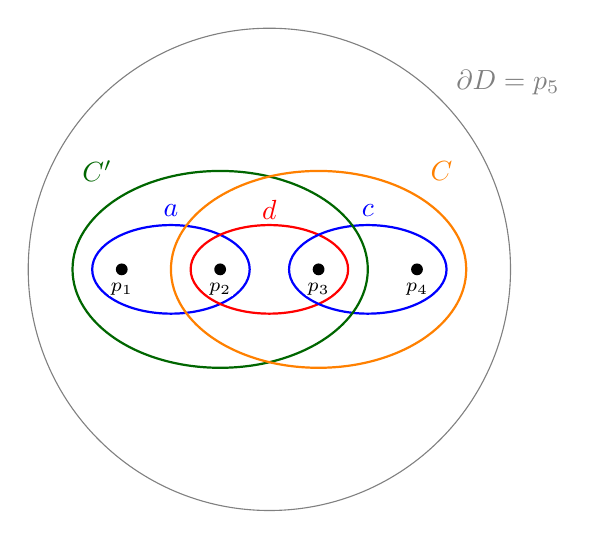
\begin{tikzpicture}[scale=1.25]
% Ellipses: centers on the x-axis, (half-width, half-height); punctures at x = 1, 2, 3, 4.
\draw[gray] (2.5,0) circle (2.45);
\draw[thick,blue] (1.5,0) ellipse (0.8 and 0.45);   % a = round{1,2}
\draw[thick,red] (2.5,0) ellipse (0.8 and 0.45);    % d = round{2,3}
\draw[thick,blue] (3.5,0) ellipse (0.8 and 0.45);   % c = round{3,4}
\draw[thick,black!60!green] (2,0) ellipse (1.5 and 1);  % C' = round{1,2,3}
\draw[thick,orange] (3,0) ellipse (1.5 and 1);      % C = round{2,3,4}
\foreach \x/\l in {1/1,2/2,3/3,4/4} {\fill (\x,0) circle (0.06); \node[fill=white,inner sep=0.5pt] at (\x,-0.2) {\scriptsize $p_\l$};}
\node[blue] at (1.5,0.6) {$a$};
\node[red] at (2.5,0.6) {$d$};
\node[blue] at (3.5,0.6) {$c$};
\node[black!60!green] at (0.75,1.0) {$C'$};
\node[orange] at (4.25,1.0) {$C$};
\node[gray,anchor=west] at (4.3,1.9) {$\partial D = p_5$};
\end{tikzpicture}
\caption{The five curves in the disk model: $D$ with four punctures
$p_1,\dots,p_4$ on a diameter, the boundary circle playing the role of the
fifth boundary component. Each curve encloses a run of consecutive
punctures: $a$, $d$, $c$ enclose $\{1,2\}$, $\{2,3\}$, $\{3,4\}$, and $C'$,
$C$ enclose $\{1,2,3\}$, $\{2,3,4\}$. In the cyclic order
$a,d,c,C',C$ consecutive curves meet twice and the others are disjoint.
The multitwist is $t=T_aT_c^{\pm1}$ (blue curves) and $f_k=T_a^kT_d$.}
\label{fig:curves}
\end{figure}

\section{The reducible-base examples}\label{sec:proof}

Cancellation gives the exceptional members in Theorem~\ref{thm:main};
a pants decomposition verifies its filling hypothesis.

\noindent\emph{Proof of Theorem~\ref{thm:main}.} We prove its three items in turn. Fix
$k\ge1$ and $\varepsilon\in\{1,-1\}$, and put $f=f_k=T_a^kT_d$ and
$t=T_aT_c^{\varepsilon}$.

\paragraph{(1) The multitwist.} By Lemma~\ref{lem:pentagon}, $a$ and $c$ are
disjoint, and they are not isotopic. Both exponents in $t$ are nonzero, and
for $\varepsilon=1$ the multitwist $t$ is a product of left twists.

\paragraph{(2) The orbits fill.} We first show that an essential curve
$\gamma$ with $i(\gamma,a)=i(\gamma,c)=0$ is isotopic to $a$ or to $c$.
Suppose it is isotopic to neither. Cutting $S$ along the disjoint curves $a$
and $c$ leaves three pairs of pants: one bounded by $a$, $p_1$, $p_2$; one by
$c$, $p_3$, $p_4$; and one by $a$, $c$, $p_5$. Realize $a$, $c$, $\gamma$ by
geodesics of a complete hyperbolic metric; distinct simple closed geodesics
are in minimal position~\cite[\S1.2]{FM}, so $\gamma$ is disjoint from
$a\cup c$ and lies in one of the three pants. By (Q) it is parallel to $a$,
to $c$ or to a puncture, which contradicts our assumption or the
essentiality of $\gamma$.

Next we compute two intersection numbers of $f(a)=T_a^kT_d(a)$. Since
$i(a,a)=i(a,c)=0$, the twist $T_a^k$ fixes $a$ and $c$ by (D). By (N) and
(I1),
\[
i(a,f(a))=i\bigl(T_a^{-k}(a),T_d(a)\bigr)=i(a,T_d(a))=i(d,a)^2=4 .
\]
By (N), $i(c,f(a))=i(T_a^{-k}(c),T_d(a))=i(c,T_d(a))$, and (I2) with
$x=d$, $y=a$, $z=c$, $m=1$ gives
$\bigl|\,i(T_d(a),c)-i(d,a)\,i(d,c)\bigr|\le i(a,c)=0$, so
$i(c,f(a))=2\cdot2=4$.

Now let $\gamma$ be any essential curve. If $\gamma$ is disjoint from both
$a$ and $c$, it is $a$ or $c$, and both meet $f(a)$. So some member of
$\{a,c,f(a)\}$ meets $\gamma$, and this set, which lies in
$A=\{f^m(a),f^m(c):m\in\Z\}$, fills $S$.

\paragraph{(3) Two exceptional members, $k$ apart.} By (D), $T_a$ and $T_c$
commute, so $t^j=T_a^jT_c^{\varepsilon j}$ and
\[
t^jf=T_a^{k+j}\,T_c^{\varepsilon j}\,T_d\qquad(j\in\Z).
\]
For $j=0$ this is $T_a^kT_d$. By Lemma~\ref{lem:pentagon},
$i(d,C')=i(a,C')=0$, so $T_d$ and $T_a$ fix $C'$ by (D), and so does
$T_a^kT_d$. For $j=-k$ it is $T_c^{-\varepsilon k}T_d$. By
Lemma~\ref{lem:pentagon}, $i(d,C)=i(c,C)=0$, so $T_d$ and $T_c$ fix $C$,
and so does $T_c^{-\varepsilon k}T_d$. Since $C$ and $C'$ are essential,
neither member is pseudo-Anosov, by (P).

\paragraph{(4) Conclusion.} For each $k\ge1$ the hypothesis of Ivanov's
question holds for $(f_k,t)$, and the set of $j$ with $t^jf_k$ not
pseudo-Anosov contains $0$ and $-k$. Any run of consecutive integers that
contains both has at least $k+1$ elements. If $N_S$ existed, taking
$k=N_S$ would give a contradiction. So no such $N_S$ exists for the sphere
with five boundary components. \qed

\begin{remark}[conventions]\label{rem:conventions}
With right-handed twists every $T_x$ becomes $T_x^{-1}$. The proof uses
only (D), (I1), (I2) and (N), which hold for both, so it applies verbatim.
Since $f\,t^j=f\,(t^jf)\,f^{-1}$, the members $ft^j$ and $t^jf$ are
conjugate and have the same exceptional $j$.
\end{remark}



\section{Pseudo-Anosov bases}\label{sec:pa}

Penner's construction proves the additional assertion in
Theorem~\ref{thm:pa}, that the base is pseudo-Anosov.

\begin{proof}[Proof of Theorem~\ref{thm:pa}]
The version of Penner's construction we use is the following
\cite[Theorem~3.1, p.~187, and definitions on pp.~180--181]{Penner}. On an oriented
finite-type surface of negative Euler characteristic, take two internally
disjoint multicurves with essential nonperipheral components, no parallel
repetitions, efficient intersections, and union filling by disks and
peripheral annuli or punctured disks. Every word in positive right twists
on the first family and negative right twists on the second is
pseudo-Anosov if every generator occurs. Here peripheral regions are parallel to an end, and efficient
intersections exclude unpunctured bigons. We now verify these qualifications. The curves $a,c$ are distinct disjoint
essential nonperipheral components, and $d$ is essential and distinct from
both. There are no parallel repetitions. Lemma~\ref{lem:pentagon} gives
$i(a,d)=i(c,d)=2$ and minimal position, with no unpunctured bigons.
The complement of $a\cup d\cup c$ has six disk faces after capping the
five ends: four singly punctured bigons, a singly punctured outer
quadrilateral, and one unpunctured quadrilateral. Equivalently, on the
compact surface its regions are five peripheral annuli and one disk.
These are exactly allowed filling regions in Penner's definition
\cite[p.~181]{Penner}; efficiency excludes unpunctured bigons
\cite[p.~180]{Penner}.

Figure~\ref{fig:penner} shows the three curves; their numerical
specification is in Appendix~\ref{app:diagram}.
The last marking represents the exterior end. These convex neighborhoods
are the actual round classes of Section~\ref{sec:curves}: an increasing
horizontal homeomorphism identifies the ordered interior markings, and
the fifth marking moves within its exterior face. Partitions alone are
not used to classify arbitrary curves. Exact crossings and facial walks
certify four crossings, eight edges after suppressing ordinary corners,
and six Jordan disk faces, with the puncture contents just listed.
The finite topology checks of this diagram are recorded in Appendix~\ref{app:diagram}.


\begin{figure}[ht]
\centering
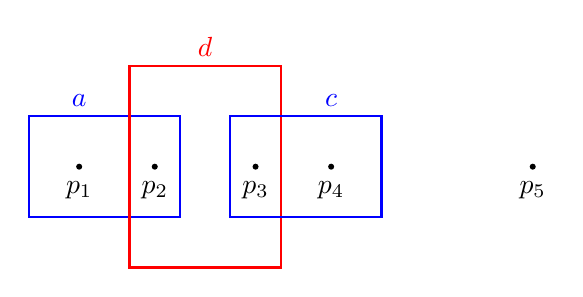
\begin{tikzpicture}[x=0.32cm,y=0.32cm]
\draw[thick,blue] (0,-2) rectangle (6,2);
\draw[thick,red] (4,-4) rectangle (10,4);
\draw[thick,blue] (8,-2) rectangle (14,2);
\foreach \x/\l in {2/1,5/2,9/3,12/4,20/5}
 {\fill (\x,0) circle (0.12); \node[below] at (\x,-0.2) {$p_\l$};}
\node[blue,above] at (2,2) {$a$};
\node[red,above] at (7,4) {$d$};
\node[blue,above] at (12,2) {$c$};
\end{tikzpicture}
\caption{The three curves used in Penner's construction, in the rational
coordinates specified in Appendix~\ref{app:diagram}. The exterior marking represents the
fifth end.}
\label{fig:penner}
\end{figure}

Penner uses right twists $\tau_x$, so our left twists satisfy
$T_x=\tau_x^{-1}$. Thus
$g_k=\tau_a\tau_c^{k+1}\tau_d^{-1}$ is in his semigroup with positive
family $\{a,c\}$ and negative family $\{d\}$. Every generator is used,
with multiplicities $1,k+1,1$, and the oriented surface has Euler
characteristic $-3$. His theorem makes $g_k$
pseudo-Anosov. Global reversal exchanges the two signed families and
preserves this conclusion.

For filling, set $M_k=T_a^{-1}T_c^{-(k+1)}$. It fixes $a,c$ by (D).
Thus $g_k=M_kT_d$.
By (N), (I1), (I2) and Lemma~\ref{lem:pentagon},
\[
 i(a,g_k(a))=i(a,T_d(a))=4,\qquad
 i(c,g_k(a))=i(c,T_d(a))=4.
\]
For the second equality the error in (I2) is at most $i(a,c)=0$.
Cutting along $a,c$ gives the three pants
$(p_1,p_2,a),(p_3,p_4,c),(a,c,p_5)$. As in the proof of
Theorem~\ref{thm:main}, an essential curve disjoint from $a,c$ is
isotopic to one of them, and hence meets $g_k(a)$. This proves filling
by the finite subfamily using only orbit indices $0,1$.

Disjoint supports give $T_aT_c=T_cT_a$, so combining integer powers
proves the displayed normal form for every $n\in\Z$. At $n=1$ it is
$T_c^{-k}T_d$, which fixes the actual $C$ since $i(c,C)=i(d,C)=0$.
At $n=k+1$ it is $T_a^kT_d$, which fixes the actual $C'$ since
$i(a,C')=i(d,C')=0$. Both reducing curves have a $2\mid3$ partition
and are essential. By (P) both members fail to be pseudo-Anosov.
The exponents are $k$ apart, so an interval containing them has at least
$k+1$ integers.
\end{proof}

\section{Computational verification}\label{sec:checks}

We relate the identities formalized in Lean to the surface argument.

\paragraph{The model.} The fundamental group of $S$ (the disk with four
punctures) is free on loops $x_1,\dots,x_4$ around $p_1,\dots,p_4$, with
$x_1x_2x_3x_4$ parallel to $\partial D$. Choosing a basepoint and representatives gives the Artin
automorphisms for half twists
\[
\sigma_i:\ x_i\mapsto x_ix_{i+1}x_i^{-1},\quad x_{i+1}\mapsto x_i,\quad
x_m\mapsto x_m\ (m\ne i,i+1),
\]
and the twists about the round curves are the full twists of the enclosed
strands~\cite[Ch.~9]{FM}: $T_a=\sigma_1^2$, $T_d=\sigma_2^2$, $T_c=\sigma_3^2$,
$T_{C'}=(\sigma_1\sigma_2)^3$, $T_C=(\sigma_2\sigma_3)^3$, up to one global
choice of handedness. The canonical fundamental-group action is only defined up to inner
automorphism; this ambiguity disappears on conjugacy classes. The five
curves are represented, up to conjugacy and inversion, by the words $x_1x_2$, $x_2x_3$, $x_3x_4$, $x_1x_2x_3$, $x_2x_3x_4$.

The group identities are formalized in Lean. Their interpretation as
statements about curves uses the standard surface facts of Section~\ref{sec:conventions}. The finite checks are given in Appendix~\ref{app:algebra}.
Here is the correspondence with
Theorem~\ref{thm:pa}. In the following displays, the twist symbols denote
the corresponding Artin endomorphisms of $F_4$. Multiplication denotes composition of
endomorphisms, with the right factor acting first. The formal definitions
are $t=T_aT_c$ and $g_k=T_a^{-1}T_c^{-(k+1)}T_d$ for
$k\in\mathbb N$, where the inverse symbols denote the specified inverse
Artin maps. Write $w_C=x_2x_3x_4$ and $w_{C'}=x_1x_2x_3$
for the words representing $C,C'$. The formal theorems
\texttt{Multitwist.V2.fixed\_C} and \texttt{Multitwist.V2.fixed\_Cp} state
\[
 ((t^1)g_k)(w_C)=w_C,\qquad
 ((t^{k+1})g_k)(w_{C'})=w_{C'}\quad(k\in\mathbb N).
\]
For Theorem~\ref{thm:main}, the formal statements
\texttt{Multitwist.F3\_j0}, \texttt{F3\_jk\_pos}, and
\texttt{F3\_jk\_neg} are, in the same notation,
\begin{gather*}
 (T_a^kT_d)(w_{C'})=w_{C'},\\
 ((T_a^{-1}T_c^{-1})^k(T_a^kT_d))(w_C)=w_C,\\
 ((T_a^{-1}T_c)^k(T_a^kT_d))(w_C)=w_C\qquad(k\in\mathbb N).
\end{gather*}
The last two equations are the two signs of the member at exponent $-k$.
The formal theorem \texttt{Multitwist.V2.}\allowbreak\texttt{integer\_identity} states,
for every group $G$, elements $A,C,D\in G$ with $AC=CA$, and
$k,n\in\mathbb Z$,
\[
 (AC)^n(A^{-1}C^{-(k+1)}D)=A^{n-1}C^{n-k-1}D.
\]
The concrete fixed-word statements use natural $k$, including zero;
the surface theorems require $k\ge1$. The integer identity supplies
the normal form for all integers $n$. Further formal nonconjugacy
statements show that the words representing $f_k(a)$ and $g_k(a)$ are
moved by the twists about $a$ and $c$, even up to conjugacy and inversion. These are the algebraic counterparts of
the positive intersection numbers used in the filling arguments.
Both choices of $\varepsilon$ occur in the displayed identities for
Theorem~\ref{thm:main}; reversing all twists is justified in
Remark~\ref{rem:conventions} and the proof of Theorem~\ref{thm:pa}. The interpretation of
Artin maps as twists, the injection of essential curve classes into
conjugacy classes up to inversion, the intersection formulas, filling,
Penner's theorem and the Nielsen--Thurston implication are supplied by the cited surface results and the topological arguments
above. The curve--word correspondence is a standard fact used here,
not a claim that it or the surface theory has been formalized. The standard logical axioms and reproduction commands
are listed in the checking notes.

\begin{appendices}
\section{Finite checks}\label{app:diagram}\label{app:algebra}

We give the numerical specifications and routine finite verifications
used alongside the main argument.

For the complementary regions, Figure~\ref{fig:penner} uses
punctures $p_1=(2,0)$, $p_2=(5,0)$, $p_3=(9,0)$, $p_4=(12,0)$,
$p_5=(20,0)$ and rectangles with coordinate
bounds
\[
 a=[0,6]\times[-2,2],\quad d=[4,10]\times[-4,4],\quad
 c=[8,14]\times[-2,2].
\]

For the diagram in Figure~\ref{fig:penner}, two independent implementations check the crossings and facial walks; neither infers the
complementary regions solely from intersection numbers.

The algebraic model in Section~\ref{sec:checks} has the following five finite facts:

\begin{itemize}
\item[F0.] Each of $T_a,T_d,T_c,T_{C'},T_C$ fixes its own curve.
\item[F1.] The pentagon pattern of Lemma~\ref{lem:pentagon}: $T_u(v)=v$ for
  the ten ordered disjoint pairs and $T_u(v)\ne v$ for the ten ordered
  meeting pairs.
\item[F2.] $T_aT_c=T_cT_a$.
\item[F3.] For every $k$ and both signs, $T_a^kT_d$ fixes $C'$ and
  $t^{-k}f_k=T_c^{-\varepsilon k}T_d$ fixes $C$.
\item[F4.] For every $k$, $T_a(f_k(a))\ne f_k(a)$ and $T_c(f_k(a))\ne f_k(a)$,
  that is, $f_k(a)$ meets $a$ and $c$.
\end{itemize}

The free-group calculation proves these facts for every natural $k$ and
both signs. It also proves the equalities and nonconjugacy statements for
$g_k$, with the formal statements displayed in Section~\ref{sec:checks}.

The independent curve calculation uses Dynnikov coordinates on the
four-punctured disk~\cite{Dynnikov}, the update rules of Hall and
Yurttaş~\cite{HY}, and the intersection formula of Yurttaş and
Hall~\cite[Lemma~9]{YH}. It confirms the pentagon pattern and the exact
intersection values $i(a,f_k(a))=i(c,f_k(a))=4$ in finite instances.
The supplementary checking notes give the exact programs, ranges,
test inputs and logical axioms.

\end{appendices}

\section*{Acknowledgments}

The preliminary checks used Mark Bell's programs \texttt{flipper} and
\texttt{curver}. \begin{thebibliography}{99}

\bibitem{BGZ} S.~Boyer, C.~McA.~Gordon and X.~Zhang, \emph{Dehn fillings of
large hyperbolic 3-manifolds}, J. Differential Geom. \textbf{58} (2001),
263--308. \doi{10.4310/jdg/1090348327}.

\bibitem{CW} M.~Cumplido and B.~Wiest, \emph{A positive proportion of
elements of mapping class groups is pseudo-Anosov}, Bull. London Math. Soc.
\textbf{50} (2018), 390--394. \doi{10.1112/blms.12148}. Posted March 15,
2017, \href{https://arxiv.org/abs/1703.05044}{arXiv:1703.05044}.

\bibitem{Dynnikov} I.~A.~Dynnikov, \emph{On a Yang--Baxter map and the
Dehornoy ordering}, Russian Math. Surveys \textbf{57} (2002), 592--594.
\doi{10.1070/RM2002v057n03ABEH000519}.

\bibitem{FM} B.~Farb and D.~Margalit, \emph{A Primer on Mapping Class
Groups}, Princeton University Press, 2012.

\bibitem{Fathi} A.~Fathi, \emph{Dehn twists and pseudo-Anosov
diffeomorphisms}, Invent. Math. \textbf{87} (1987), 129--151.
\doi{10.1007/BF01389156}.

\bibitem{FLP} A.~Fathi, F.~Laudenbach and V.~Poénaru, \emph{Travaux de
Thurston sur les surfaces}, Astérisque \textbf{66--67}, 1979.

\bibitem{HY} T.~Hall and S.~Ö.~Yurttaş, \emph{On the topological entropy of
families of braids}, Topology Appl. \textbf{156} (2009), 1554--1564.
\doi{10.1016/j.topol.2009.01.005}. \href{https://arxiv.org/abs/0808.3053}{arXiv:0808.3053}.

\bibitem{Ivanov94} N.~V.~Ivanov, \emph{Ten problems on the mapping class
groups}, headed 1994--1998, 2014 (original version early 1994,
updates to 1998, retypeset 2014); posted on the author's website,
\url{https://nikolaivivanov.com/wp-content/uploads/2014/02/ivanov1994problems.pdf}.

\bibitem{Ivanov06} N.~V.~Ivanov, \emph{Fifteen problems about the mapping
class groups}, in \emph{Problems on Mapping Class Groups and Related
Topics}, Proc. Sympos. Pure Math. \textbf{74}, Amer. Math. Soc., 2006,
71--80. \doi{10.1090/pspum/074/2264532}. Posted August 14, 2006,
\href{https://arxiv.org/abs/math/0608325}{arXiv:math/0608325}.

\bibitem{LM} D.~D.~Long and H.~R.~Morton, \emph{Hyperbolic 3-manifolds and
surface automorphisms}, Topology \textbf{25} (1986), 575--583.
\doi{10.1016/0040-9383(86)90033-9}.

\bibitem{Penner} R.~C.~Penner, \emph{A construction of pseudo-Anosov
homeomorphisms}, Trans. Amer. Math. Soc. \textbf{310} (1988), 179--197.
\doi{10.1090/S0002-9947-1988-0930079-9}.

\bibitem{Watanabe} Y.~Watanabe, \emph{Pseudo-Anosov mapping classes from
pure mapping classes}, Trans. Amer. Math. Soc. \textbf{373} (2020),
419--434. \doi{10.1090/tran/7919}. Posted November 16, 2016,
\href{https://arxiv.org/abs/1611.05119}{arXiv:1611.05119}.

\bibitem{YH} S.~Ö.~Yurttaş and T.~Hall, \emph{Intersections of multicurves
from Dynnikov coordinates}, Bull. Aust. Math. Soc. \textbf{98} (2018),
149--158. \doi{10.1017/S0004972718000308}.
\href{https://arxiv.org/abs/1711.00895}{arXiv:1711.00895}.

\bibitem{Zhang07} C.~Zhang, \emph{Some pseudo-Anosov maps on punctured
Riemann surfaces represented by multi-twists}, preprint, first posted
August 6, 2007, \href{https://arxiv.org/abs/0708.0804v1}{arXiv:0708.0804v1};
withdrawn by the author (version 2, January 16, 2008).

\bibitem{Zhang11} C.~Zhang, \emph{Dehn twists combined with pseudo-Anosov
maps}, Kodai Math. J. \textbf{34} (2011), 367--382.
\doi{10.2996/kmj/1320935547}.

\end{thebibliography}
\end{document}
